\documentclass[12pt]{report}
\usepackage[english]{babel}
\usepackage[utf8]{inputenc}
\usepackage[ruled,vlined,linesnumbered]{algorithm2e}
\usepackage{graphicx}
\usepackage{caption}
\usepackage{amsmath}
\usepackage{hyperref}

\begin{document}

\begin{titlepage}
\begin{center}

\hfill

\bigskip
\huge{Université de Bordeaux \par \Large Projet d'Etude et de Recherche} 
\vfill
\bigskip 
\Huge 
\bigskip Efficient, Proximity-Preserving Node Overlap Removal \par 
\vfill
\Large Claire Pennarun \par 
		Tatiana Rocher
\vfill
\Large Article by E.R. Gansner and Y. Hu (2009)	
		\bigskip 
\bigskip

\Large
\today
\end{center}
\end{titlepage}

\tableofcontents
\newpage

% abstract

\chapter{Subject presentation and state of the art}

%Partie "domaine general : graph drawing"
A graph is a data structure encoding information with the use of nodes and edges (which are binary relations between nodes).

Graph drawing aims to represent a given information as a graph, generally through a "node-link" layout, letting only nodes and edges be displayed. 

\bigskip
%Partie "domaine specifique : node overlap + etat de l'art"
Most of the layout algorithms consider nodes as points, but some need to let appear additional information as labels. For example, London subway maps would be useless without the indication of the stations on the lines.

This could lead to an overlap of some nodes. That must be avoided, as it clearly confuses the understanding of the graph.

Moreover, as we generally consider that the original layout contains significant information, an other parameter to deal with is to maintain the "global shape" of the initial representation. 

This "global shape" can be seen as "preserving the proximity relations between nodes", "preserving the orthogonal ordering of nodes"(see \cite{Mis95}) or "preserving the relative positions of nodes by limiting the vertices displacement"(see \cite{Gansner98}), and a choice between these criteria has to be made.

The easiest approach is to "scale" the layout until no overlaps occur. This method has the advantage to preserve the global shape of the layout, but the area of the graph can become very inconvenient. That is why a compromise between the preservation of the "shape of the graph" and a minimization of the total area has to be found.

Different algorithms have been devised to answer the problem, each of them focusing on a different "global shape" definition. 

\bigskip
The first approach is to try to avoid overlaps while generating the layout.

The spring-electrical model presented by Eades \cite{Eades84} and Fruchterman and Reingold \cite{FR91} considers the edges as springs between nodes, so that the spring forces move the nodes to a minimal energy state of the global system. A repelling force between non-adjacent nodes is added.
This model has been adapted by various authors (\cite{HK02}, \cite{Li05}) to take the node size into account, generally as increased repulsive forces.

The stress model of Kamada and Kawai \cite{Kamada89} is based on the assumption that a graph layout is "good" if the distance between two vertices is close to the theoretical graph distance between these vertices, i.e. to the length of their shortest path. It can also be extended to avoid as much as possible overlap along the edges.

These two models (spring-electrical model and stress model) try to avoid all overlaps, but use generally a post-processing algorithm to ensure the total overlap removal.

More details about the force-directed drawing algorithms can be found in \cite{Kob13}.

\bigskip
The second possibility is to remove overlaps after the graph is drawn : these are post-processing algorithms.

The Voronoi cluster busting algorithm \cite{Gansner98} restrains the possible displacement of a node with the use of Voronoi cells. This restriction aims to help preserving the relative positions of the nodes. In practice, the algorithm often requires a lot of iterations and the global similarity with the initial layout can be low (see for example the figure \ref{voronoi}).

\begin{figure}[h]
  \setlength\fboxsep{5pt}
  \setlength\fboxrule{0.5pt}
  \fbox{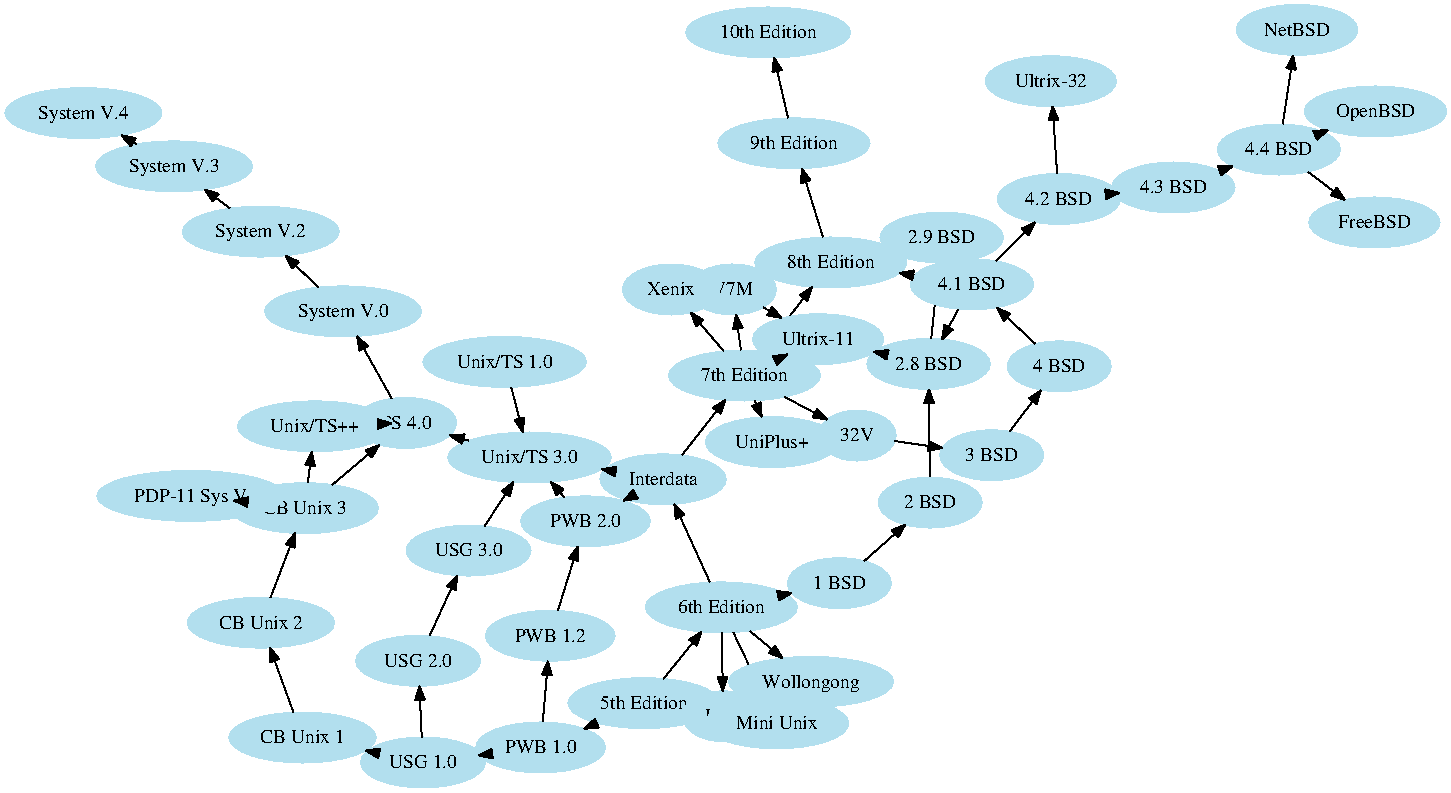
\includegraphics[width=0.425\textwidth]{figures/size.png}}
  \fbox{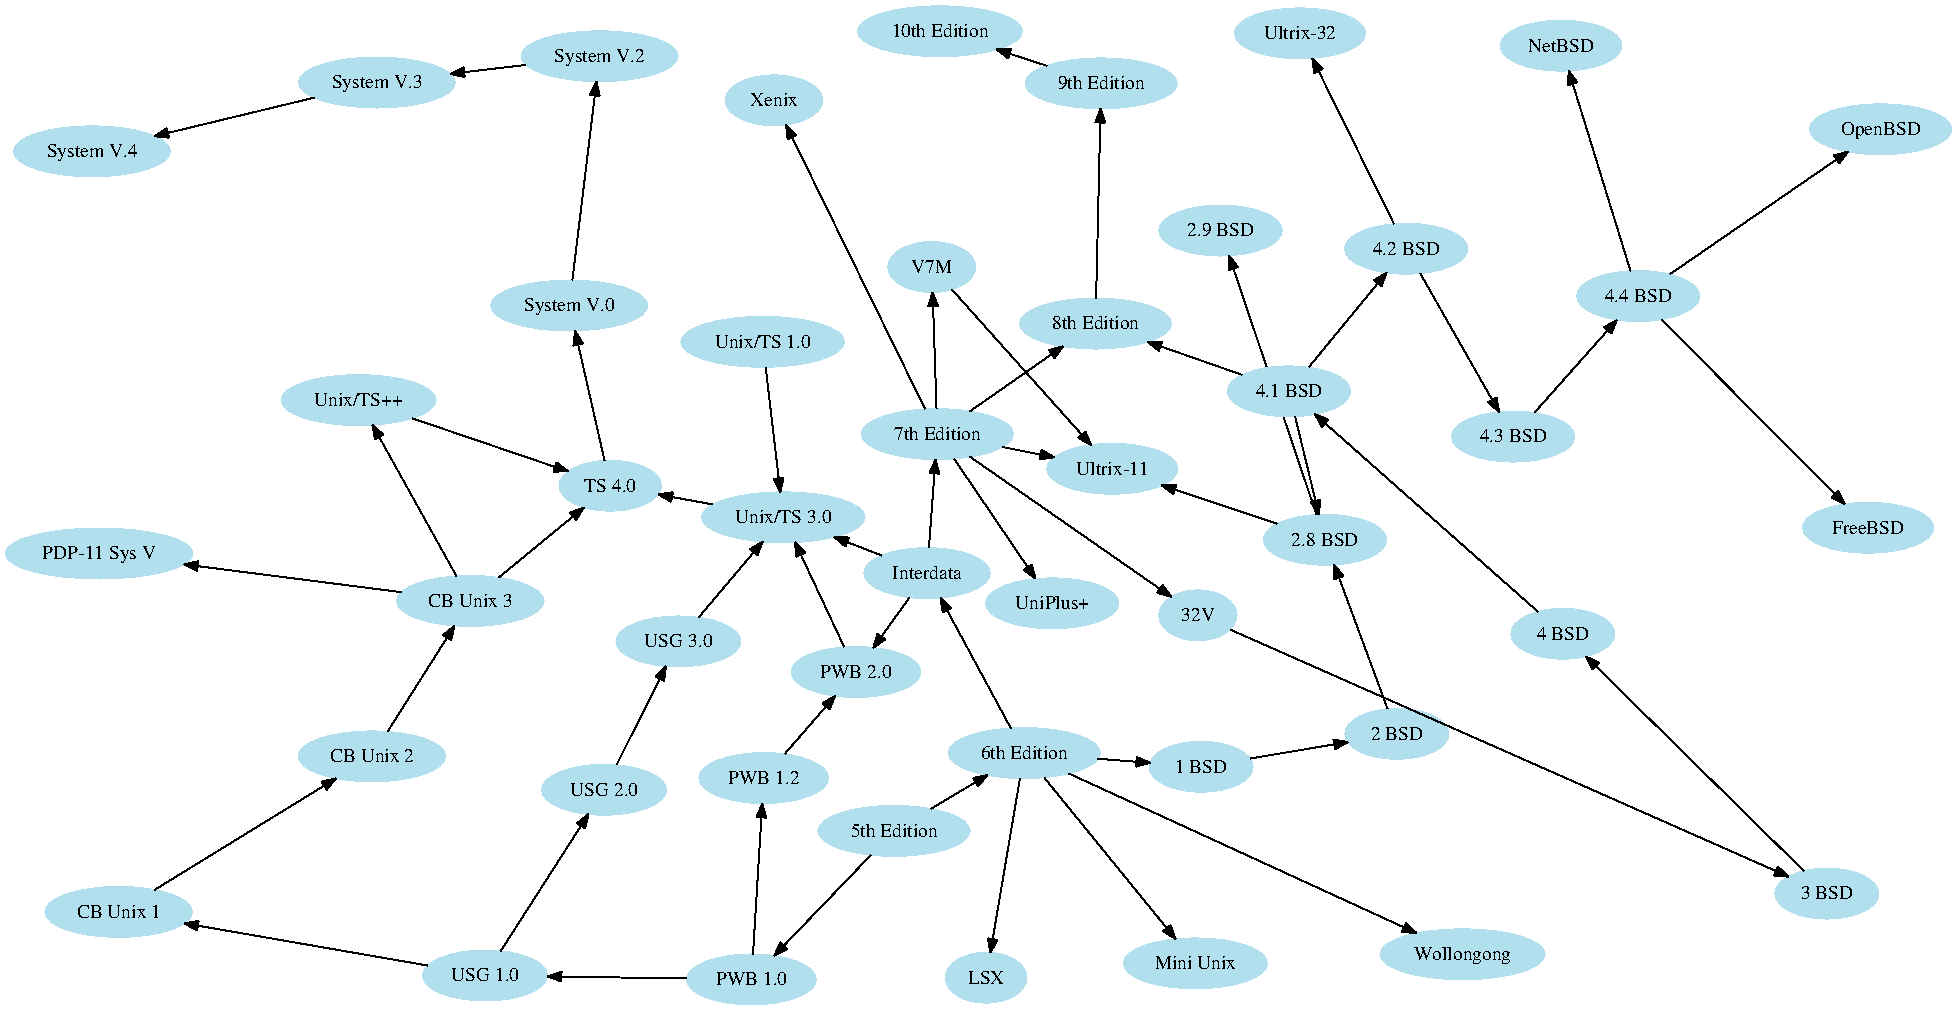
\includegraphics[width=0.45\textwidth]{figures/sizeVoro.png}}
  \caption{(left) The initial layout. (right) The result of the Voronoi-based algorithm}
  \label{voronoi}
\end{figure}
%% modifier image ?

The Satisfy\_VPSC algorithm \cite{VPSC06}, solving the "variable placements with separation constraints" problem, moves iteratively the nodes in the horizontal and in the vertical dimensions. This algorithm aims to minimize the vertices displacement but can generate layouts that are very dissimilar to the initial layout. %(mettre exemples)

Some work on word cloud generators like Wordle (\url{http://www.wordle.net/}) allowed to develop new algorithms like Mani-Wordle \cite{Koh10} and RWordle \cite{SSSK12} based on a spiral scheme for the random placement of text labels in order to overcome overlaps.


\bigskip
%Partie : "presentation du projet"
Our project consists in understanding the algorithm PRISM proposed by Gansner and Hu in \cite{Gansner08} and in analyzing the feasability of its implementation as a plugin for the Tulip software \cite{Auber12}.

% Bien expliquer pourquoi on veut garder les relations de proximité



\chapter{PRISM algorithm}

\section{Formal notations}

We use the following notations : $G = (V,E)$ denotes the current graph, with $V$ the set of vertices (or nodes), and $E$ the set of edges. The number of vertices and of edges are denoted respectively $|V|$ (or $n$) and $|E|$.

An edge between two vertices $i$ and $j$ is denoted $(i,j)$.

The position of a node $i$ in a layout is represented as a set of 2D coordinates $p_i = (x_i, y_i)$. The initial layout position of $i$ is denoted as $p_i^0 = (x_i^0, y_i^0)$.

We consider for the PRISM algorithm that a node $i$ has a certain width $w_i$ and height $h_i$, thus forming a rectangle containing the label, likely to cause overlaps.

\section{Description of the algorithm}

The PRISM algorithm focuses on two main constraints for the final layout of the graph. First, the area taken by the layout must be minimal. The second constraint is to preserve the global "shape" of the original layout by maintaining all proximity relations between the nodes.

The PRISM algorithm runs in two main steps ; in a first step, it removes iteratively the overlaps between near nodes of the given graph $G$. Then it finds the non-near overlapping nodes and removes these overlaps as well.

\subsection{Overlap removal between near nodes}

\subsubsection{Use of a proximity graph - Delaunay Triangulation}

To find easily the overlaps between near nodes of the graph $G$, it will efficient to work on a proximity graph of $G$. Such a graph will also guarantee the preservation of the proximity relations during the different stages of the algorithm.

A \emph{proximity graph} is a graph in which two vertices are connected by an edge if (and only if) they satisfy a given geometrical property (a survey on proximity graphs can be found in \cite{JT92}).

\bigskip

The \emph{Delaunay triangulation} (DT) (named after the work of Delaunay \cite{Delaunay34}) of a graph $G$ is a triangulation of the graph such that none of the circumscribed circles of the triangles in DT(G) contains a vertex on the inside. This particular triangulation also maximises the minimum angle of the triangles found.

\begin{figure}[h]
	\center
  \setlength\fboxsep{5pt}
  \setlength\fboxrule{0.5pt}
  \fbox{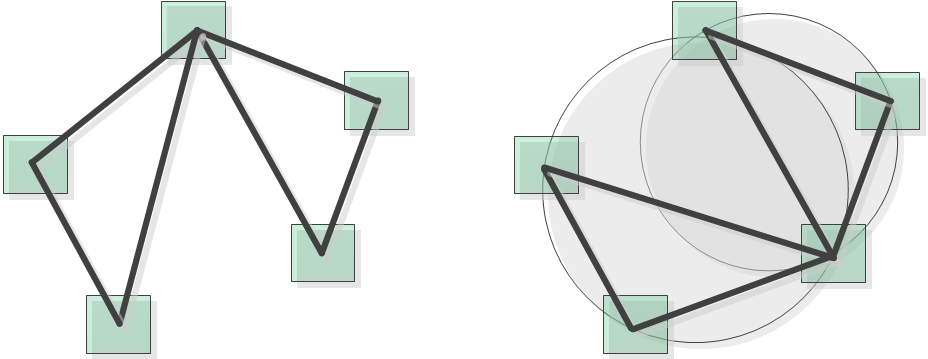
\includegraphics[width=0.5\textwidth]{figures/DT.png}}
  \caption{(left) A graph $G$. (right) The Delaunay triangulation of $G$}
  \label{DT}
\end{figure}
%% modifier image ?

The Delaunay triangulation of $G$, as a triangulation, is also a planar graph, and has thus at most $3n -6$ edges (if $|V(G)| = n$), which is a very practical parameter for the algorithm.

\bigskip

The nearest neighbors of a vertex $v \in V(G)$ tend to form triangles with $v$ and in particular, the closest neighbor of $v$ has an edge with $v$ in DT(G), as the nearest neighbor graph of $G$ is a subgraph of DT(G) (see \cite{JT92}).

In the PRISM algorithm, we consider that the near nodes in $G$ are connected by an edge in the Delaunay triangulation of $G$.

Thus, the algorithm's first goal is to remove overlaps along the edges of the Delaunay triangulation of $G$.

\subsubsection{Ideal edge length}
The idea is to find the "ideal length" of the Delaunay triangulation edges : the "ideal length" of an edge is such that the two edge ends have no overlap.

\bigskip
In order to do that, we calculate an \emph{overlap factor} $f_{ij}$ for each edge $(i,j)$ ($i,j \in V(G)$) of the Delaunay triangulation of $G$ :

\[ f_{ij} = \max \left( \min \left(\frac{w_i/2 + w_j/2}{x_i - x_j}, 
\frac{h_i/2 + h_j/2}{y_i - y_j} \right), 1 \right)\]

where $(x_i,y_i)$ are the coordinates of vertex $i$, $w_i$ its width and $h_i$ its height.

If two nodes $i$ and $j$ have no overlap, then $f_{ij} = 1$. 
If $i$ and $j$ do overlap, then that overlap can be removed by expanding the edge $(i,j)$ by the overlap factor found $f_{ij}$ (see figure \ref{overlapFactor}). 

\begin{figure}[h]
	\center
  \setlength\fboxsep{5pt}
  \setlength\fboxrule{0.5pt}
  \fbox{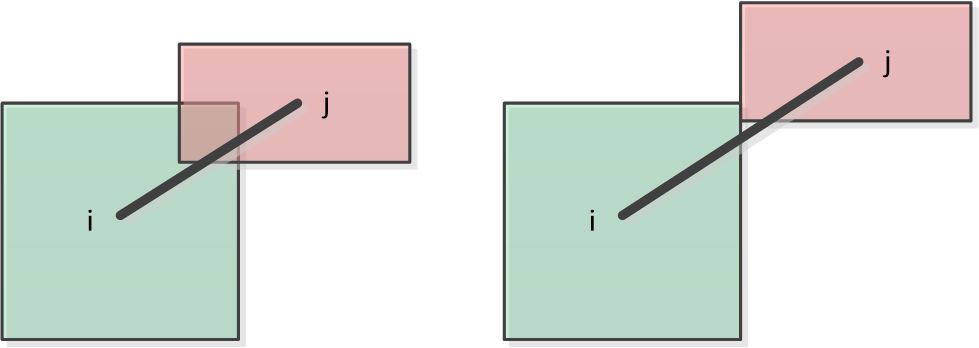
\includegraphics[width=0.5\textwidth]{figures/FacteurChevauchement.png}}
  \caption{Overlap factor}
  \label{overlapFactor}
\end{figure}
%% modifier image ?

Thus, the "ideal length" of an edge of the Delaunay triangulation is $l_{ij} = f_{ij}||p_i^0 - p_j^0||$, where $p_i^0$ is the initial set of coordinates of a node $i$.

We now want to find coordinates for the nodes of the initial graph such that the edges length in $DT(G)$ are close to their ideal length.

\subsubsection{Proximity stress model}

Finding this new set of coordinates means minimizing the following sum :

\[ E = \sum_{i,j \in E(DT(G))} w_{ij}(||p_i - p_j|| - l_{ij})^2\]

where $l_{ij}$ is the overlap factor and $w_{ij} = 1/(l_{ij})^2$ is a classic weighting factor, used to equalize the contributions to the total sum from the different edges.

But there are some situations where keeping $l_{ij}$ is not a good idea (see figure \ref{badcase}).

\begin{figure}[h]
	\center
  \setlength\fboxsep{5pt}
  \setlength\fboxrule{0.5pt}
  \fbox{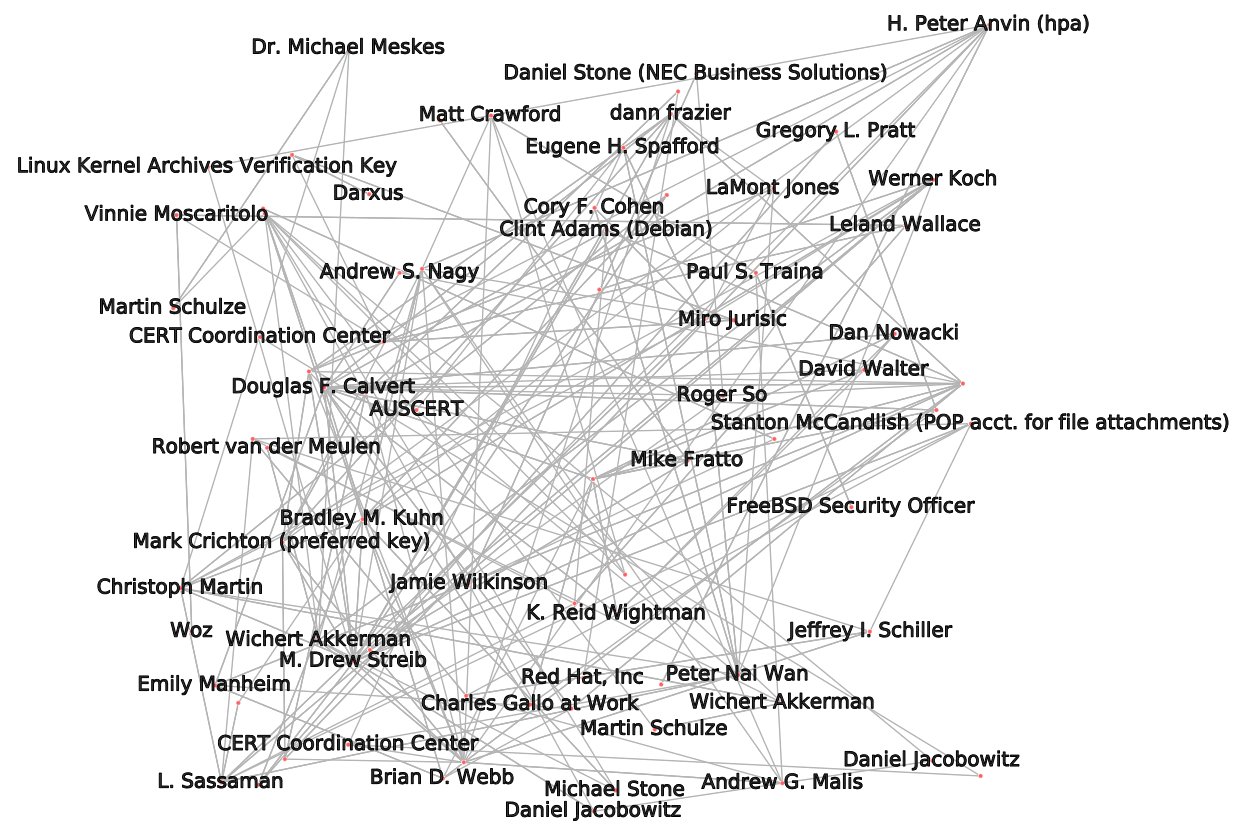
\includegraphics[width=0.5\textwidth]{figures/graphTulip0.png}}
  \caption{A bad case}
  \label{badcase}
\end{figure}
%% modifier image !

We thus want to avoid removing the "big" overlaps in one iteration only.
So we have to replace $f_{ij}$ by $\min(f_{ij},s)$, where $s > 1$ will be a limiting factor. The authors found that $s = 1.5$ worked well.

This type of sum is called a "stress function", in analogy with the well studied \emph{stress model} introduced by Kruskal in \cite{Kruskal64} and applied to graph drawing by Kamada and Kawai in \cite{Kamada89}. 
The above sum is called the \emph{proximity stress model}.

\bigskip
The minimization of the sum gives new positions for the nodes of $G$.

\subsubsection{Iteration and termination}
This first phase provides us with a new layout of the graph $G$, in which the nodes positions are given according to the previous minimization of the proximity stress model.

This layout may still contain overlaps. We must thus iterate the construction of the Delaunay triangulation, the computation of the overlap factors, the minimization of the proximity stress model and the move of the nodes until no more overlaps occur along the edges of the Delaunay triangulation of the graph.

\bigskip
The process of the first stage makes clear that no overlaps can appear : the distance between nodes can only be increasing and the proximity graph on which we are calculating, as a triangulation, is a rigid graph.

But the authors do not explain formally the reason of the termination of this phase : the stress function could always be smaller but never reach a local minimum. Moreover, the number of iterations needed during the first phase is not explicited nor bounded in the article.

The authors' implementation of PRISM contains a threshold : if the gain in the minimization of the stress function is smaller, the first phase of the algorithm ends.

%% A preciser et detailler

\subsection{Overlap removal between non-near nodes}

The first step removes the overlap between ends of edges of the Delaunay triangulation of the graph. But some overlaps can be caused by nodes not being near, and thus not generating an edge in the proximity graph. These overlaps can not have been removed by the first stage of the PRISM algorithm.

To find these still overlapping nodes, we have to use a scan-line algorithm.

\subsubsection{Scan-line algorithm}

A scan-line algorithm is an algorithm which will consider all the points of a layout.

We can not use a algorithm which uses the graph properties because the vertices do not know the positions of others vertices, so we can not find the overlaps by using the vertices properties.

For all the ordinate's points we consider all the points in the abscissa. If there is an overlap at a point, we add the edge (between the two vertices overlapping) in the Delaunay triangulation. 
% à etoffer


\bigskip
It is interesting to note that one of the opponent algorithms, Satisfy\_VPSC \cite{VPSC06}, mainly uses a scan-line algorithm to remove overlaps.

\subsubsection{Overlap removal}

The second stage uses the same processus as the first one, only adding the overlapping edges found by the scan-line algorithm to the Delaunay triangulation before the calculation of the overlap factors and the resolution of the proximity stress model.

This stage ends when no more overlaps are found by the scan-line algorithm.
% A completer ?

\begin{figure}
\begin{algorithm}[H]
\caption{PRISM}
\KwIn{$p_i^0$ : coordinates of each vertex  \\
	 width $w_i$ and height $h_i$ of each vertex ($i = 1,2,...,|V|$)}
	 
\Repeat{}{$G_{DT}$ : proximity graph of $G$ by Delaunay triangulation \\
	\For{all edges of $G_{DT}$}
	{Compute the overlap factor}
	$\{p_i\}$ : solution of the proximity stress model
	
	$p_i^0 = p_i$
}	
(no more overlaps along edges of $G_{DT}$)
\BlankLine
\Repeat{}{$G_{DT}$ : proximity graph of $G$ by Delaunay triangulation \\
	Find overlaps in $G$ through a scan-line algorithm \\
	Add the overlapping edges to $G_{DT}$ \\
	\For{all edges of $G_{DT}$}
	{Compute the overlap factor}
	$\{p_i\}$ : solution of the proximity stress model
	
	$p_i^0 = p_i$
}	
(no more overlaps found by the scan-line algorithm)
\end{algorithm}
\caption{The PRISM algorithm}
\end{figure}

\subsection{Dissimilarity metrics}

To be able to compare different graph layouts, the authors propose three dissimilarity metrics : the area taken by the layout, a metric based on the edge length ratio in the proximity graphs of the initial and final layouts, and a metric measuring the vertices displacement between the initial and the final layouts.

\subsubsection{Area}
As said before, it is easy to remove all the overlaps by extending all the edges of the initial layout. But the final layout can be extremely large and thus unreadable, so we want to keep an area as small as possible.

\subsubsection{Edge length ratio}
We first calculate the ratio between the edge lengths of the proximity graphs of the original layout and the final one. The metric is then defined as the normalized standard deviation to the mean ratio found.

This metric has to be as small as possible to minimize the changes made to the edges length during the algorithm.

The edge length ratio has to be calculated on a rigid graph (as the Delaunay triangulations) to be meaningful : two layouts of the same graph can be completely different if the graph is not rigid. (exemple ?)

\subsubsection{Vertices displacement}

The third measure of dissimilarity is the calculation of the displacement of vertices between the original layout and the final one. We consider that layouts resulting from a scaling, a shift or a rotation are identical. Thus, computing the displacement of vertices means finding the optimal scaling, shift and rotation minimizing the displacement. (formule ?)

\section{Complexity}


$\rightarrow$ comparaison avec VPSC
\chapter{Implementation within Tulip}

\section{The Tulip framework}

The Tulip framework \cite{Auber12}, developed mainly by the Data Visualization team of the LaBRI (Bordeaux), is a data visualization software dedicated to the analysis and visualization of relational data. It focuses on the manipulation of graphs. Our goal was to implement the PRISM algorithm as a plugin for Tulip, reusing some of the tools already present in the software, such as the calculation of the Delaunay triangulation of a graph.

Tulip uses particular structures to deal with graph manipulations, and one of these structure is very important for the PRISM algorithm : the \texttt{node} structure.

The PRISM algorithm considers that the label is part of the node, and that the size of the node is determined by the size of the underlying label.

But in Tulip, the labels are seen as a "property" of the graph, and are decorrelated from the nodes themselves. They generally are dynamic sized, and displayed in order to avoid overlaps. We thus do not have access to the size of labels.

The solution was to increase the size of the nodes and to force the labels inside them (see figure \ref{graphTulip}). Thus, we could considerate that the "labels" were overlapping, even if it was artificially.

\begin{figure}[h]
  \setlength\fboxsep{5pt}
  \setlength\fboxrule{0.5pt}
  \fbox{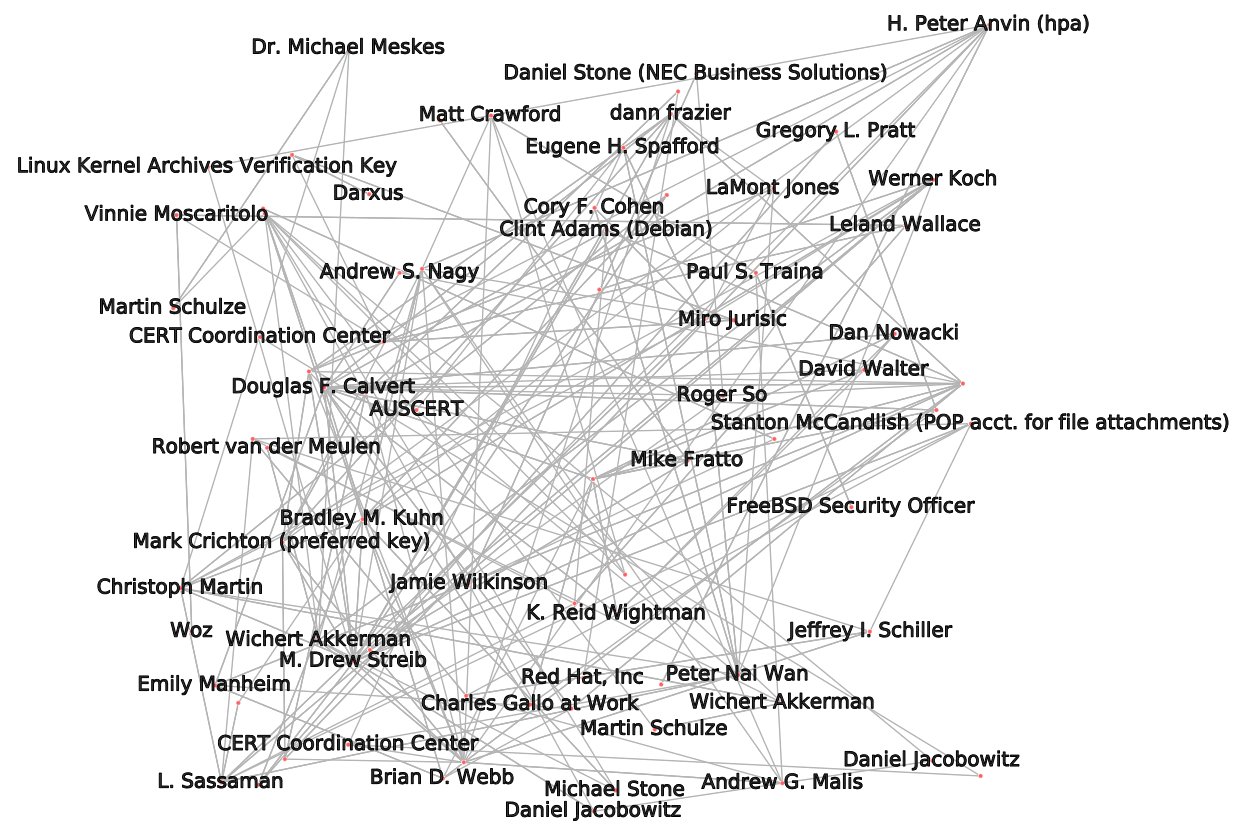
\includegraphics[width=0.5\textwidth]{figures/graphTulip0.png}}
  \fbox{
\includegraphics[width=0.5\textwidth]{figures/graphTulipWithLabels0.png}}
  \caption{Adjustment of the nodes size in Tulip}
  \label{graphTulip}
\end{figure}

\section{Resolution of the stress model}

The resolution of the proximity stress model can be done in many different ways. The authors, through their implementation in GraphViz \cite{Gansner02}, a set of graph drawing tools, chose to solve it via a stress majorization technique (described in details in \cite{Gansner05}). 

\subsubsection{Stress majorization}

We first considered to implement the resolution of the proximity stress model in the same way as the authors by employing a stress majorization technique.

This procedure consists in bounding the function we want to optimize by a series of quadratic functions from above. Solving the stress model means then finding an optimum, which is done by solving a series of linear systems.

\bigskip
This resolution implies the manipulation of weighted Laplacian of matrices and the use of a conjugate gradient algorithm with preconditions. These features are not present in the Tulip framework and were too complex to implement in the given time for the project. 

\bigskip
Another possibility was to retrieve some implementation from the GraphViz suite and use it as an external plugin or module. 
But a analysis of the dependencies of the requested function (the \texttt{StressMajorizationSmoother\_smooth()} function in the \texttt{post\_process.c} file) were to important to do so.

The python script used to retrieve these dependancies is given as an annex (mettre ref)

\bigskip
We then focused on finding an other resolution method for the proximity stress model and we decided to adapt an algorithm based on a Newton-Raphson method.

\subsubsection{Newton-Raphson method - Kamada \& Kawai}

Kamada and Kawai \cite{Kamada89} proposed an algorithm computing a local minimum of the energy $E$ of a system. We adapted and implemented it by using 
\[ E = \sum_{i,j \in E(DT(G))} w_{ij}(||p_i - p_j|| - l_{ij})^2 \]
The purpose is to calculate new positions $p_i = (x_i, y_i)$ for $i = 1... n$, locally minimizing the global stress function $E$. 

We thus want to find $x_i, y_i$ such that $\delta E / \delta x_i = \delta E / \delta y_i = 0$ for $i = 1... n$. That means solving simultaneously $2n$ (non-linear) equations.

\bigskip
The Kamada and Kawai algorithm consists in moving only one node $i$ at a time to reach $\delta E / \delta x_i = \delta E / \delta y_i = 0$, "freezing" the other nodes during the computation.

We adapted the computation of $\delta E / \delta x_i$ and $\delta E / \delta y_i$ to our configuration : we considered the following values :

\begin{eqnarray*}
\frac{\delta^2 E}{\delta x_i}  & = & \sum_{(i,m) \in E(DT)} w_{im} ( (x_m - x_i) - \frac{l_{im} (x_m - x_i)}{||p_m - p_i||} \\
\frac{\delta^2 E}{\delta y_i}  & = & \sum_{(i,m) \in E(DT)} w_{im} ( (y_m - y_i) - \frac{l_{im} (y_m - y_i)}{||p_m - p_i||}
\end{eqnarray*}
 
where $DT$ is the Delaunay triangulation of the graph, $l_{im}$ is the ideal length of the $(i,m)$ edge, $w_{im} = 1/(l_{im})^2 $ is a weighting factor, and $||p_m - p_i||$ is the euclidian distance between the nodes $m$ and $i$.

At each iteration, the node moved is the one having the largest value of $\Delta_i$ (i.e. the "further" one of the condition to reach):

\[\Delta_i = \sqrt{\left(\frac{\delta E}{\delta x_i}\right)^2 + \left(\frac{\delta E}{\delta y_i}\right)^2} \]


\bigskip
We thus only have to solve a two-equations system at each step (the two unknown values are $\delta x$ and $\delta y$):
\begin{eqnarray*}
\frac{\delta^2 E}{\delta x_i^2}(p_i) \times \delta x +  \frac{\delta^2 E}{\delta x_i \delta y_i}(p_i) \times \delta y  & = & - \frac{\delta E}{\delta x_i} (p_i) \\
\frac{\delta^2 E}{\delta y_i \delta x_i}(p_i) \times \delta x +  \frac{\delta^2 E}{\delta y_i^2}(p_i) \times \delta y & = & - \frac{\delta E}{\delta y_i} (p_i)
\end{eqnarray*}

The $(\delta x, \delta y)$ found are added to the current position of the node $i$, and this is done iteratively until $\Delta_i < \varepsilon$, where $\varepsilon$ is a threshold determined by the user.

The algorithm stops when all considered nodes have reached $\Delta_i < \varepsilon$. As $\varepsilon \neq 0$, it happens that all nodes have not been removed.

\section{Scan-line algorithm}
Implementation details

\section{Tests and results}
Tests and time of the Kamada and Kawai solution

\chapter{Conclusion}

Since PRISM :

ePRISM : PRISM on overlap of edges \cite{Hu09}

\bibliographystyle{plain}
\bibliography{report_prism}

\end{document}
